

\subsection{Prototypische Implementierung des Anwendungsfalls}

In diesem Kapitel wird die Umsetzung des entwickelten Prototypen im Detail beschrieben.
Zunächst wird die Erzeugung eines cyberphysischen Systems als Industrie-4.0-Komponente beschrieben. Im Anschluss wird dargestellt, wie Daten des Messinstruments über die \textit{Internet of Things Edge Platform} an die SAP Cloud Platform übergeben werden. Daraufhin wird die Erzeugung eines digitalen Zwilllings und die Zuordnung von Funktionen beschrieben. Abschließend wird dargestellt, wie der Zustand der Anlage den Nutzern in einer UI5-Applikation präsentiert werden.

\subsubsection{Erzeugung eines cyberphysischen Systems}

Für die Simulation einer Windergieanlage wird ein System erzeugt, welches Daten aus der Umwelt aufnehmen und verarbeiten kann. Bei den Daten wurde sich für die \textit{Windgeschwindigkeit, Temperatur, Luftfeuchtigkeit, Luftdruck und Luftdichte} entschieden.
Als hardwareseitige Basis für die Simulation wird ein \textit{Raspberry Pi 3 B} verwendet, welcher die erstellten \textit{Python} Skripte zur Verarbeitung der Daten nutzt. Der Pi wurde um die Zusatzplatine \textit{Grove Pi + Board} erweitert. Somit wird der \textit{DHT11}-Sensor zur Messung von Temperatur und Luftfeuchtigkeit über die 4-Pin-Schnittstelle \textit{D4} einfach ohne Löten und Breadboard angebunden. Für die Messung der Windgeschwindigkeit ist die Entscheidung auf den Anemometer \textit{Eltako Windsensor WS} gefallen. Im Gegensatz zum \textit{DHT11-Sensor} ist der Anenometer ein aktives Mechanisches Gerät, dessen Output Berechnungen erfordert, um die Windgeschwindigkeit zu erhalten. Bei den ausgegebenen Signalen handelt es sich um die Berührung zweier Metallkontakte, wobei zwei Signale eine Umdrehung ergeben. Ein Python Skript zählt die Signale über der GPIO-4-Schnittstelle und berechnet die Geschwindigkeit für ein Zeitintervall von 5 Sekunden. Aufgrund mangelhafter Sensorik wird der Luftdruck aus einem Array von realistischen Werten zufällig pro Zeitintervall ausgewählt. Gemeinsam mit der gemessenen Temperatur und dem Luftdruck wird die Luftdichte berechnet. Bevor die Daten an das Gateway gesendet werden, werden sie dem String-Dictionary \textit{sensorData} übergeben, um eine Anfrage im \textit{JSON-Format} senden zu können. Außerdem wurde eine rote Grove-LED über die digitale Schnittstelle D3 angebunden. Diese Komponente dient im Gegensatz zu den weiteren Komponenten dazu, bei kritischen Temperaturwerten Befehle zum Aufleuchten zu erhalten. Damit soll gezeigt werden, dass sich der Kreis in einem cyberphysischen System von Sensorik bis Aktorik über SAP Leoanardo als informationsverarbeitende Schicht schließt.

\begin{figure}[H]
  \centering
  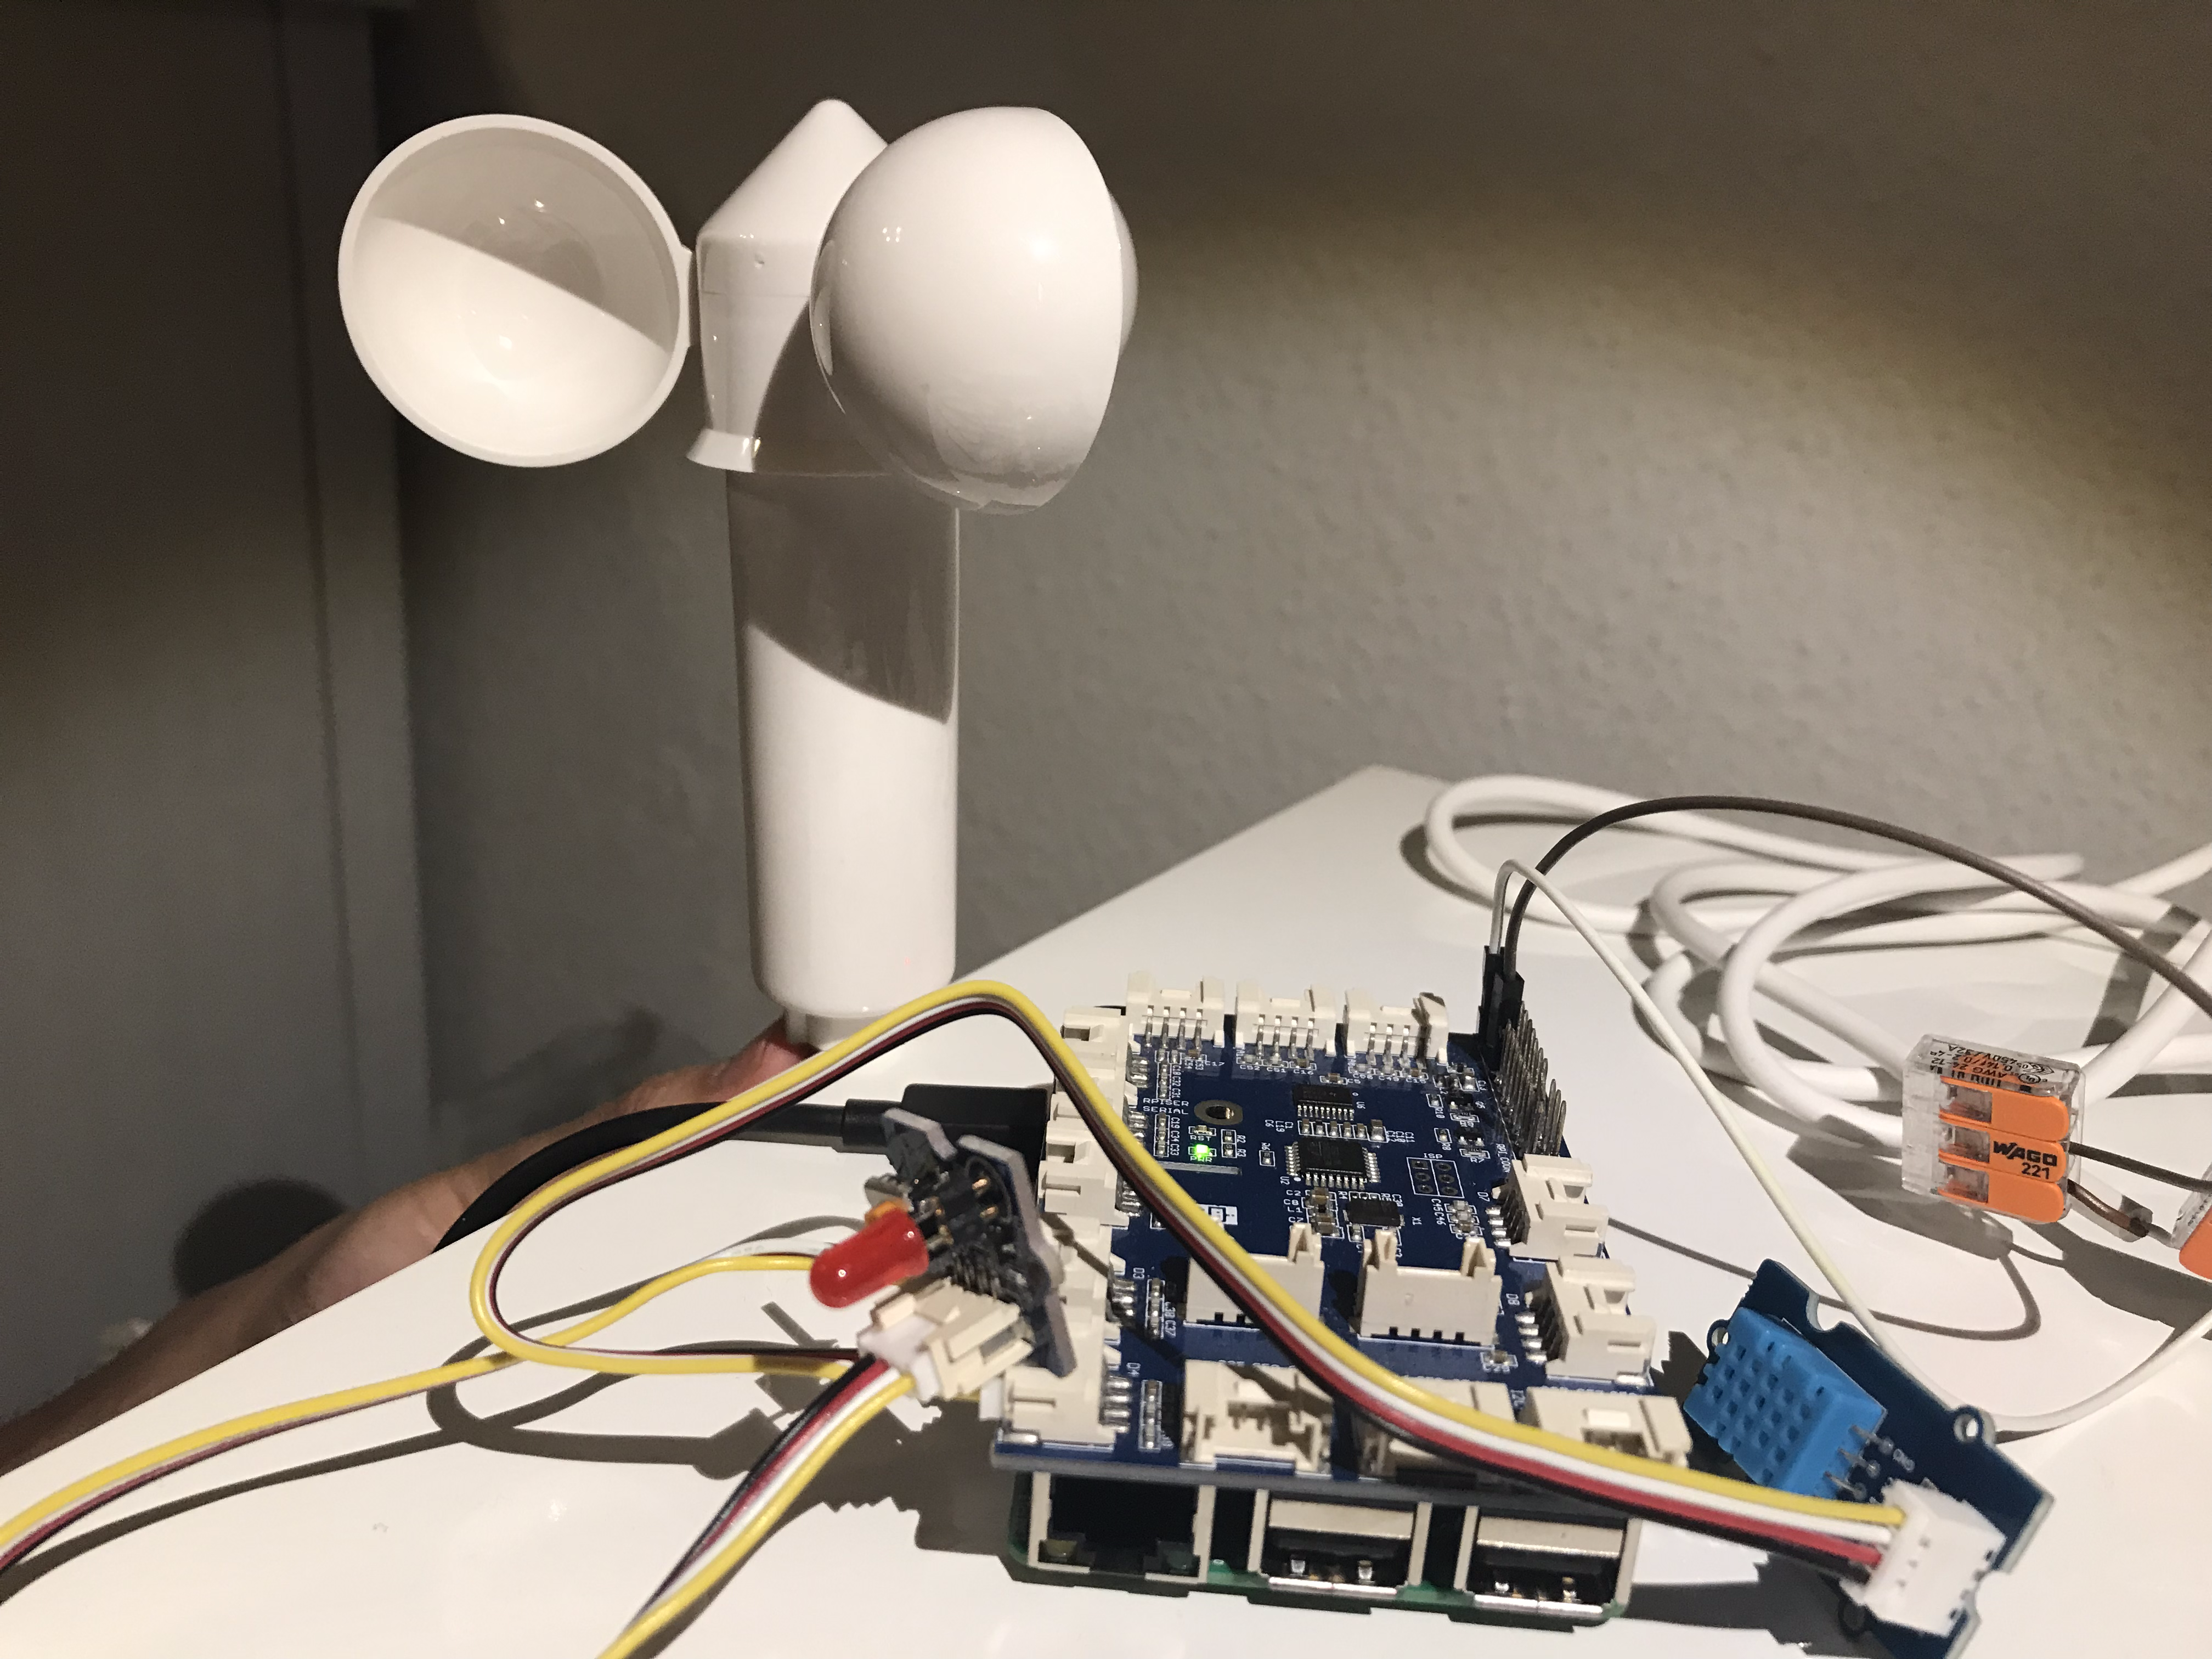
\includegraphics[width=1\linewidth]{prototype.png}
  \caption[Cyberphysisches System für die Simulation]{Cyberphysisches System für die Simulation (eigene Darstellung)}
  \label{raspi}
\end{figure}


\subsubsection{Einrichtung der Gateway Edge}

Damit die aufgenommenen Sensorwerte zur Datenhaltung an den \textit{Internet of Things Service} gesendet werden können, muss ein Gateway existieren. Doch anstatt die vordefinierten Cloud Gateways im \textit{IoT Service Cockpit} zu nutzen, wird für den Prototypen ein lokales Edge Gateway des \textit{REST}-Protokolls mit Hilfe der \textit{Internet of Things Edge Platform} konfiguriert. Zunächst wird aus dem SAP Software Center eine Konfigurationsdatei heruntergeladen, welche auf dem Raspberry Pi lokal gespeichert wird. Mit dem Befehl \textit{./build.sh REST} werden weitere Konfigurationsdateien erzeugt, um die Verbindung zu dem Host des Internet of Things Service herzustellen. In der Datei \textit{config\_gateway\_rest.xml} wird der Endpunkt für den Datentransfer in einer \textit{ConnectionAddress} definiert und eine \textit{GatewayAlternateId} definiert.

\begin{lstlisting}[caption= Gateway-Verbindung zur Cloud]
  <cnf:address>https://5075f8b9-866e-4a4b-82f8-74687b72f1ab.eu10.cp.iot.sap:443/5075f8b9-866e-4a4b-82f8-74687b72f1ab/iot/core/api/v1/tenant/988439498</cnf:address>
  <cnf:gateway gatewayAlternateId="1122334455667788">
\end{lstlisting}
Als Serveradresse des Edge Gateways wird die IP-Adresse des Raspberry Pi angegeben. Somit ist die Zieladresse für die Sensordaten zum Beispiel:

\begin{lstlisting}[caption= Zieladresse für Sensorwerte]
  https://192.168.178.52:8699/measures/<deviceAlternateId>\end{lstlisting}

\noindent Abschließend benötigt die Gateway-Registierung einen \textit{private Key im pem-Format}.

\begin{lstlisting}[caption= GET-Anfrage für einen Client-Key]
curl -X GET "https://5075f8b9-866e-4a4b-82f8-74687b72f1ab.eu10.cp.iot.sap/5075f8b9-866e-4a4b-82f8-74687b72f1ab/iot/core/api/v1/tenants/988439498/gatewayRegistrations/clientCertificate/pem\end{lstlisting}

\noindent Nach dem Starten des Gateways auf dem Raspberry Pi mit dem Befehl \textit{./gateway.sh} wird folgendes Gateway initialisiert:

\begin{lstlisting}[caption= Gateway-Eigenschaften]
  {
  "id": "2019161729",
  "alternateId": "1122334455667788",
  "protocolId": "rest",
  "name": "IoT Gateway REST",
  "type": "edge",
  "creationTimestamp": 1571741372988,
  "status": "online",
  "version": "4.42.0",
  "operatingSystem": "Linux;4.19.75-v7+;arm"
}\end{lstlisting}

\subsubsection{Registrierung der Geräte}

Bevor die Daten von der SAP Cloud Platform aufgenommen werden können, muss eine Instanz eines Gerätetypen erstellt werden. Die Registrierung folgt dem vordefinierten Datenmodell aus Abbildung \ref{fig:devicemodel} und wird mit POST-Anfragen an die \textit{Device Management API} durchgeführt. Zunächst wird mit die \textit{Capability wind\_1} vom Typ \textit{measure} erstellt. Der Capability werden die \textit{Properties wind\_speed, temperature, humidity, pressure und airtight} zugeordnet. Damit das Gerät Befehle empfangen kann, wird außerdem die Capability \textit{commands\_test} vom Typ \textit{command} erstellt. Anschließend werden beide Capabilities einem Sensortypen zugeordnet. Um jedoch eine Geräteinstant erzeugen zu können, muss eine
mit SAP Cloud Platform Internet of Things und Device Model hier erstellen und als Bild einfügen und außerdem zunächst auf Tenants und User eingehen und Einrichtungs des Services generell erklären mit eventuell den Message Processings
und Gateways etc



\subsubsection{Senden der Daten an die Cloud}

\begin{lstlisting}
============================================
Reading sensor data ...
{'capabilityAlternateId': '1234', 'measures': [{'temperature': '19.0'}, {'wind_speed': '1.12102078977'}, {'pressure': '1010'}, {'humidity': '70.0'}, {'airtight': '1.2'}], 'sensorAlternateId': '1234'}
==> HTTP Response: 202
\end{lstlisting}

\subsubsection{Erstellen des digitalen Zwillings}

\paragraph{Regeln, Ereignisse, Aktionen}

AWS, Events, LED Commands und Destinations
\subsubsection{Visualisierung mit einer UI5-Applikation}


\subsubsection{Zusammenfassung Implementierung}

\newpage
